\documentclass[11pt]{article}

\usepackage[margin=1in]{geometry}
\usepackage{amsmath}
\usepackage{booktabs}
\usepackage{siunitx}
\usepackage{caption}
\usepackage{pgfplots}
\pgfplotsset{compat=1.18}
\usepackage{hyperref}
\usepackage{float}

\sisetup{round-mode=places, round-precision=4, scientific-notation=true}

\title{\textbf{CSE402: Numerical Analysis, Simulation and Modeling Sessional}\\Simplified Newton--Raphson Power-Flow Implementation\\
\large (Kulworawanichpong, 2010)}
\author{Anika Morshed\\
Diganta Saha Tirtha\\
Add kore ne\\
}
\date{\today}

\begin{document}
\maketitle


\section{Overview}
Place holder for now\\


\section{Bus Admittance Matrix}
Table~\ref{tab:ybus} compares the computed bus admittance matrix $Y_{bus}$
against the matrix printed in Section 4 of the paper. Agreement is to the four
decimal places the paper itself reports; the residual \texttt{abs\_err\_mag}
is consistent with the paper's own rounding, not with a modelling error.

\begin{table}[h]
\centering
\caption{Computed vs.\ paper $Y_{bus}$ entries (magnitude in p.u., angle in degrees).}
\label{tab:ybus}
\begin{tabular}{l S[table-format=2.5] S[table-format=2.4] S[table-format=-4.5] S[table-format=-4.2] S[scientific-notation=true]}
\toprule
{Entry} & {Computed mag.} & {Paper mag.} & {Computed ang.} & {Paper ang.} & {Abs.\ error (mag.)} \\
\midrule
$Y_{11}$ & 53.85165 & 53.8517 & -68.19859 & -68.20 & 5.19287e-05 \\
$Y_{12}$ & 22.36068 & 22.3607 & 116.56505 & 116.57 & 2.02250e-05 \\
$Y_{13}$ & 31.62278 & 31.6228 & 108.43495 & 108.43 & 2.33983e-05 \\
$Y_{22}$ & 58.13777 & 58.1378 & -63.43495 & -63.43 & 3.25850e-05 \\
$Y_{23}$ & 35.77709 & 35.7771 & 116.56505 & 116.57 & 1.23600e-05 \\
$Y_{33}$ & 67.23095 & 67.2310 & -67.24902 & -67.25 & 5.47441e-05 \\
\bottomrule
\end{tabular}
\end{table}

\section{Iteration-by-Iteration Reproduction}
Table~\ref{tab:iterations} checks the current mismatch vector $F$, the
Jacobian $J$, and the correction vector $\Delta x$ produced by the PNR
solver at each of the paper's three worked iterations, against the values
printed in Section 4. \texttt{max\_abs\_diff} is the largest entry-wise
difference; \texttt{max\_rel\_diff} normalises that difference by the largest
entry of the paper's own vector or matrix, absorbing the paper's four-decimal
rounding.

\begin{table}[h]
\centering
\caption{Per-iteration agreement with Section 4 of the paper.}
\label{tab:iterations}
\begin{tabular}{c l S[scientific-notation=true] S[scientific-notation=true]}
\toprule
{Iteration} & {Quantity} & {Max.\ abs.\ diff.} & {Max.\ rel.\ diff.} \\
\midrule
1 & mismatch & 2.30769e-05 & 8.06885e-06 \\
1 & Jacobian & 0.00000e+00 & 0.00000e+00 \\
1 & $\Delta x$ & 3.65613e-05 & 7.94812e-04 \\
2 & mismatch & 4.33705e-05 & 5.25067e-04 \\
2 & Jacobian & 4.20418e-05 & 6.64784e-07 \\
2 & $\Delta x$ & 4.24941e-05 & 3.86310e-02 \\
3 & mismatch & 4.31065e-07 & 1.06964e-03 \\
3 & Jacobian & 3.88991e-05 & 6.14610e-07 \\
3 & $\Delta x$ & 3.75201e-08 & 3.67844e-03 \\
\bottomrule
\end{tabular}
\end{table}

\section{Converged Solution (Paper's Table 2)}
Table~\ref{tab:table2} compares the converged solution of both methods
(standard NR, SNR, and the proposed method, PNR) against the paper's own
Table 2. This work iterates to a $10^{-10}$ p.u.\ voltage tolerance, tighter
than the paper's own \SI{1e-6}{} p.u.\ criterion and the three hand iterations
the paper prints; the small residual gap in the angle columns reflects the
paper reporting an intermediate (third-iteration) value rather than a fully
converged one.

\begin{table}[h]
\centering
\caption{Paper Table 2 -- power-flow solution for the 3-bus example.}
\label{tab:table2}
\begin{tabular}{l S[table-format=-1.6] S[table-format=-1.5] S[table-format=-1.6] S[table-format=-1.5]}
\toprule
{Item} & {SNR (this work)} & {SNR (paper)} & {PNR (this work)} & {PNR (paper)} \\
\midrule
$|V_2|$ (p.u.)     & 0.971680  & 0.97168 & 0.971680  & 0.97168 \\
$\delta_2$ (deg)   & -2.696454 & -2.696  & -2.696454 & -2.698  \\
$|V_3|$ (p.u.)     & 1.040000  & 1.04000 & 1.040000  & 1.04000 \\
$\delta_3$ (deg)   & -0.498803 & -0.4988 & -0.498803 & -0.4979 \\
$Q_3$ (p.u.)       & 1.461769  & 1.46170 & 1.461769  & 1.46180 \\
\bottomrule
\end{tabular}
\end{table}

\section{Solution Convergence (Paper's Figure 4)}
\begin{figure}[H]
    \centering    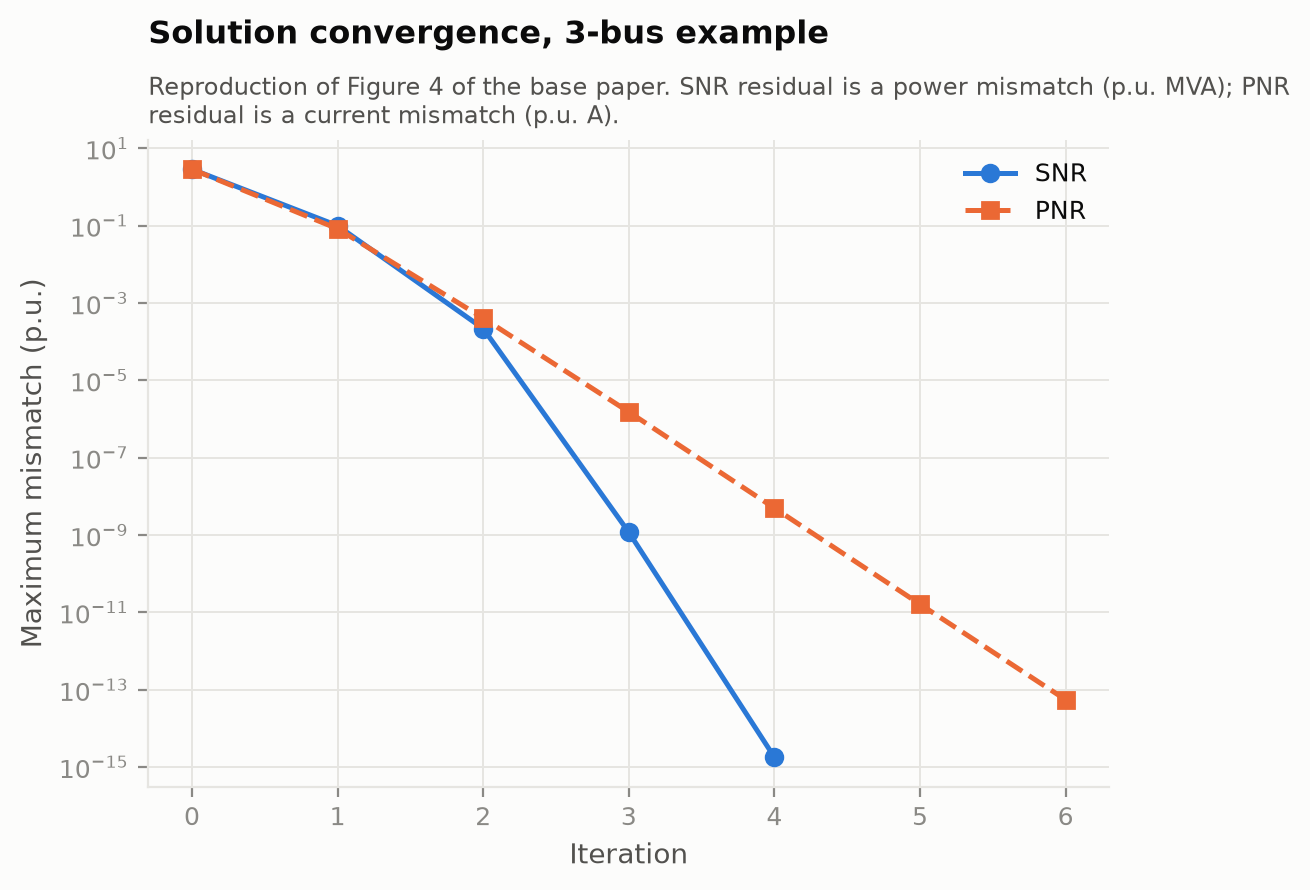
\includegraphics[width=0.8\linewidth]{results/figures/01_fig4_convergence.png}
    \caption{Caption}
    \label{fig:convergence}
\end{figure}
Figure~\ref{fig:convergence} reproduces the paper's Figure 4: the maximum
mismatch at each iteration for both methods, on a logarithmic scale. The SNR
residual is a maximum power mismatch (p.u.\ MVA); the PNR residual is a
maximum current mismatch (p.u.\ A). Both series show the characteristic
roughly-doubling number of correct digits per iteration associated with
quadratic Newton convergence; PNR requires two additional iterations to reach
machine precision, consistent with its reactive power at the PV bus being
re-estimated from the current voltage guess at the start of every iteration
rather than solved for directly.


%% ===================================================================
%%  Computational cost analysis and alternative solution methods
%% ===================================================================

\section{Per-Iteration Cost: Reproducing Section 3 of the Paper}
The paper's central claim is not that the simplified method converges in fewer
iterations --- it does not --- but that each iteration is cheaper, because the
current-mismatch Jacobian entries of equations (9), (11), (13) and (15) are much
simpler expressions than their power-mismatch counterparts. Section 3 of the
paper supports this with symbolic multiplication counts (its Table 1) and two
log--log plots (its Figures 1 and 2). Following the paper's own convention, a
``FLOP'' here is a multiplication or a division; additions, subtractions and
transcendental evaluations are treated as free.

These counts are implemented in \texttt{src/powerflow/flops.py}, which provides
three independent counting models --- \texttt{paper}, \texttt{audited} and
\texttt{sparse} --- and are driven by \texttt{scripts/02\_flop\_counting.py}.
Table~\ref{tab:table1} reproduces the totals of the paper's Table 1. Every
symbolic form is recovered exactly: $3(n-1)$ and $3(n-1)(n-2)$ for the diagonal
and off-diagonal blocks of $J_1$ and $J_3$ under standard NR, $2(n-1)+3$ and
$2(n-1)(n-2)$ for $J_2$ and $J_4$, against $4(n-2)$ diagonal and $2(n-2)$ or
$(n-2)$ off-diagonal for the proposed method.

\begin{table}[H]
\centering
\caption{Paper Table 1 -- multiplications per iteration to build the Jacobian,
as published, evaluated at each test-system size.}
\label{tab:table1}
\begin{tabular}{r r r r}
\toprule
{$n$} & {SNR total} & {PNR total} & {Claimed ratio} \\
\midrule
5    & 166       & 66     & 2.5   \\
6    & 256       & 88     & 2.9   \\
24   & 5\,296    & 484    & 10.9  \\
30   & 8\,416    & 616    & 13.7  \\
57   & 31\,366   & 1\,210 & 25.9  \\
118  & 136\,896  & 2\,552 & 53.6  \\
300  & 894\,016  & 6\,556 & 136.4 \\
\bottomrule
\end{tabular}
\end{table}

Figures~\ref{fig:flops-jacobian} and~\ref{fig:flops-mismatch} reproduce the
paper's Figures 1 and 2 on the same logarithmic axes: the Jacobian cost is
$10n^{2}$ for the standard method against $22(n-2)$ for the proposed one, and
the mismatch-vector cost is $6n$ against $4n+4$. The published claim is
therefore that the Jacobian rebuild drops from quadratic to \emph{linear} in the
bus count.

\begin{figure}[H]
    \centering
    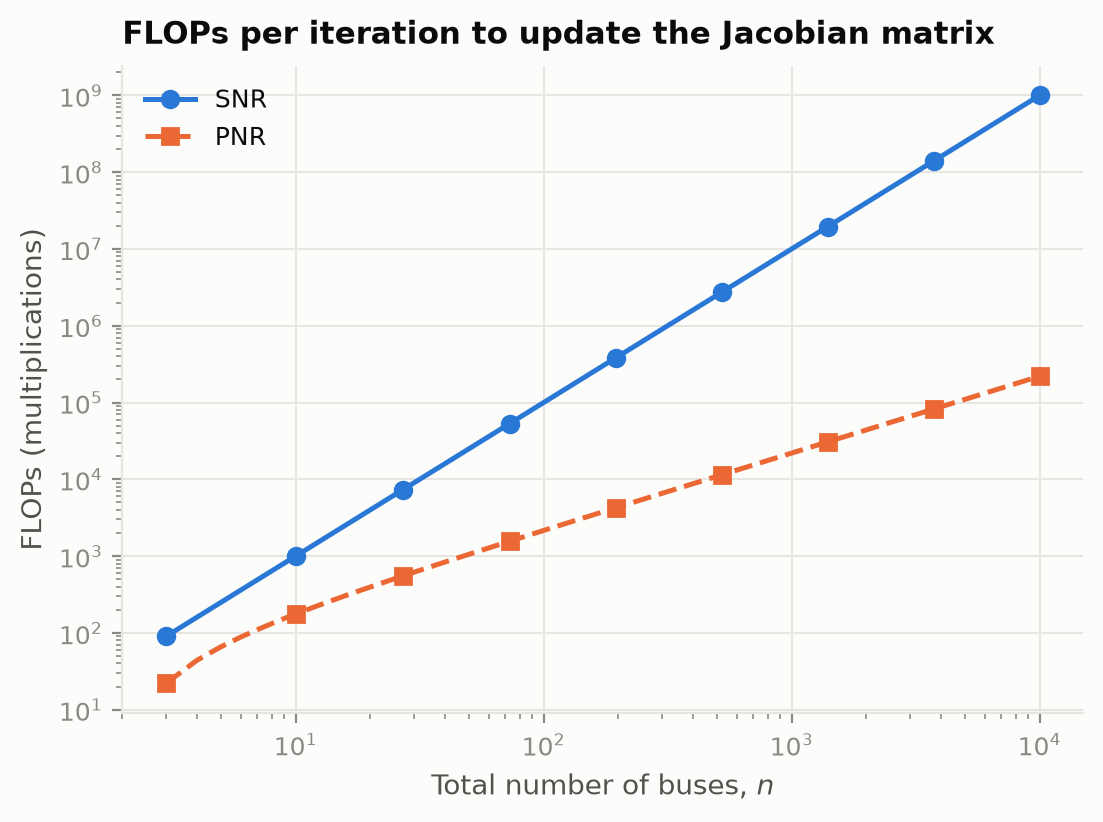
\includegraphics[width=0.72\linewidth]{results/figures/02_fig1_jacobian_flops.png}
    \caption{Paper Figure 1 reproduced: multiplications per iteration to update
    the Jacobian, $10n^{2}$ (SNR) against $22(n-2)$ (PNR).}
    \label{fig:flops-jacobian}
\end{figure}

\begin{figure}[H]
    \centering
    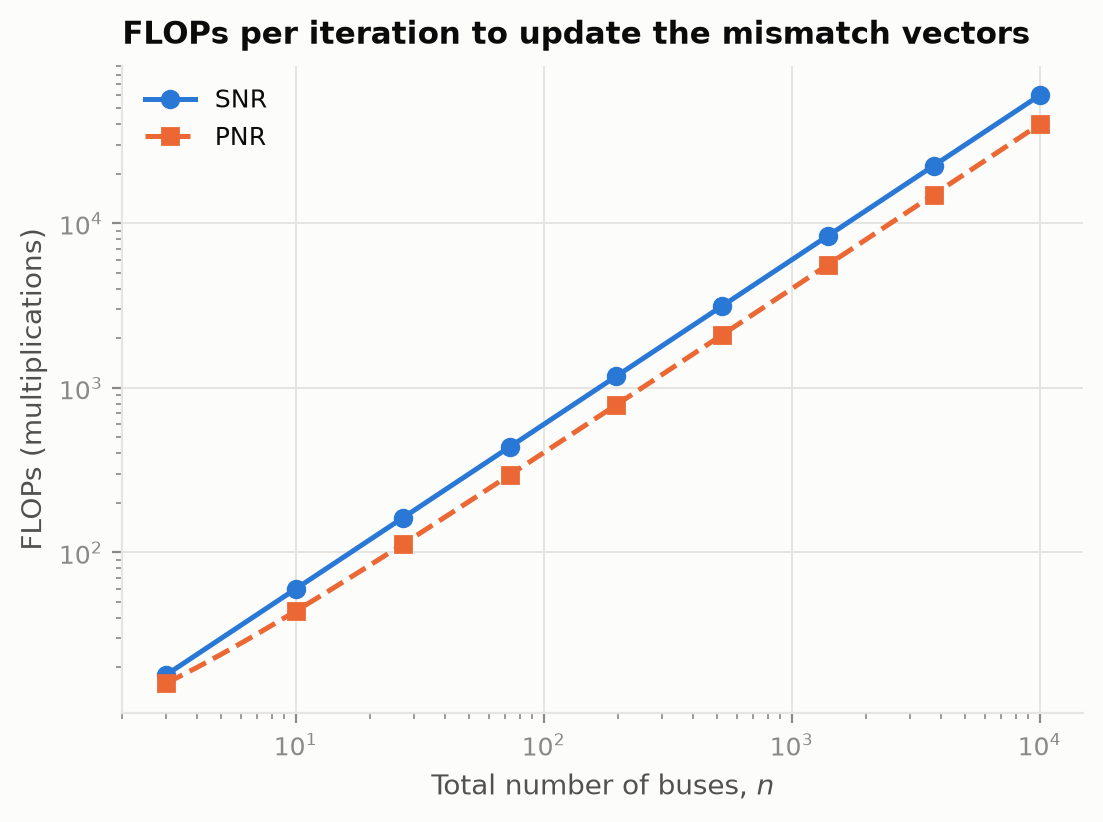
\includegraphics[width=0.72\linewidth]{results/figures/02_fig2_mismatch_flops.png}
    \caption{Paper Figure 2 reproduced: multiplications per iteration to update
    the mismatch vectors, $6n$ (SNR) against $4n+4$ (PNR).}
    \label{fig:flops-mismatch}
\end{figure}

\section{An Audited Recount of the Paper's Own Formulas}
The published counts reproduce, but they cannot be correct as stated. A dense
Jacobian has $O(n^{2})$ entries, and equations (9), (11), (13) and (15) give
every one of them a distinct admittance $Y_{ki}$, so each entry needs at least
one multiplication of its own. A cost linear in $n$ is impossible for a dense
matrix. Table 1 appears to count the off-diagonal work once per \emph{row}
rather than once per \emph{entry}, which is exactly what collapses
$(n-1)(n-2)$ into $(n-2)$.

To test whether the paper's \emph{conclusion} survives its arithmetic, the same
formulas were recounted element by element, with the identical
common-subexpression reuse granted to both methods. For an off-diagonal pair
$(k,i)$ the standard method must form $u=|V_i||Y_{ki}|$, $w=|V_k||Y_{ki}|$ and
$m=|V_k|u$ and then multiply by $\sin\alpha$ and $\cos\alpha$ where
$\alpha=\theta_{ki}+\delta_i-\delta_k$, filling all four sub-matrices and their
row sums: nine multiplications. The simplified summand carries no $|V_k|$
factor and no $-\delta_k$ in its angle, so only $u$ is needed and the count
falls to five. Against that, the simplified diagonals are closed-form
expressions (equations 10, 12, 14, 16) rather than row sums the standard method
accumulates for free, so they cost thirteen multiplications per bus against
four. Table~\ref{tab:audit-unit} collects the unit costs.

\begin{table}[H]
\centering
\caption{Audited multiplication counts per matrix element.}
\label{tab:audit-unit}
\begin{tabular}{l r r r}
\toprule
{Method} & {Per off-diagonal pair} & {Per bus (diagonals)} & {Per mismatch term} \\
\midrule
Standard NR (SNR)   & 9 & 4  & 4 \\
Simplified NR (PNR) & 5 & 13 & 3 \\
\bottomrule
\end{tabular}
\end{table}

The consequence is a constant-factor saving, not an asymptotic one. Both
methods remain $O(n^{2})$, and the predicted ratio tends to $9/5=1.80$ for the
Jacobian alone; including the mismatch vectors, which save only $4{:}3$, pulls
the combined figure down to about $1.62$. Table~\ref{tab:flop-models} sets the
published ratio beside the audited one, and Figure~\ref{fig:flop-models} plots
both models together.

\begin{table}[H]
\centering
\caption{Per-iteration cost ratio SNR${}/{}$PNR: as published versus audited.}
\label{tab:flop-models}
\begin{tabular}{r r r r r}
\toprule
{$n$} & {Audited SNR} & {Audited PNR} & {Audited ratio} & {Published ratio} \\
\midrule
5     & 192          & 163         & 1.18 & 3.1   \\
6     & 304          & 243         & 1.25 & 3.4   \\
24    & 6\,766       & 4\,419      & 1.53 & 10.1  \\
30    & 10\,792      & 6\,963      & 1.55 & 12.4  \\
57    & 40\,492      & 25\,539     & 1.59 & 22.8  \\
118   & 177\,376     & 110\,451    & 1.61 & 46.2  \\
300   & 1\,160\,722  & 717\,603    & 1.62 & 116.2 \\
1000  & 12\,969\,022 & 7\,992\,003 & 1.62 & 385.4 \\
\bottomrule
\end{tabular}
\end{table}

\begin{figure}[H]
    \centering
    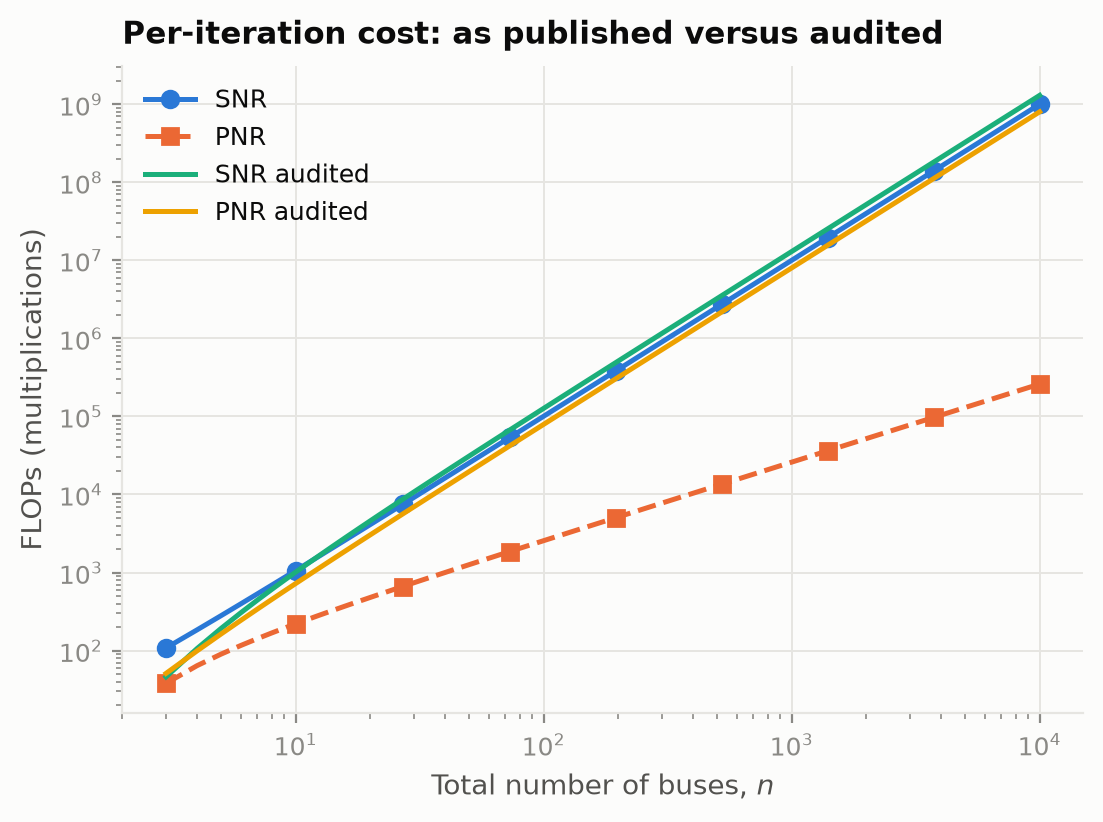
\includegraphics[width=0.72\linewidth]{results/figures/02_flop_models.png}
    \caption{Per-iteration cost as published against the audited recount of the
    same formulas. The published PNR curve is linear in $n$; the audited one is
    quadratic and parallel to SNR, separated by a constant factor.}
    \label{fig:flop-models}
\end{figure}

This is the useful result of the exercise, and it is a favourable one. For the
Jacobian alone the audited model predicts a ratio of $1.733$ at the $57$-bus
size of the paper's largest test case --- against the $1.728$ the paper actually
\emph{measured} there. The measurement the paper reports is therefore consistent
with the audited count to three significant figures, and inconsistent with its
own Table 1, which would have predicted a factor of $25.9$. The paper's
conclusion survives in full even though its Table 1 does not.

\section{Cost over the True Y-bus Sparsity Pattern}
The counts above, like the paper's, assume a dense Jacobian. Real networks are
not dense, and any practical solver stores only the non-zeros of $Y_{bus}$.
Replacing the dense off-diagonal population $(n-1)(n-2)$ with the true non-zero
count gives the third counting model. Table~\ref{tab:sparse-flops} applies it to
every test system used in this project.

\begin{table}[H]
\centering
\caption{Audited FLOP counts over the true $Y_{bus}$ sparsity pattern.}
\label{tab:sparse-flops}
\begin{tabular}{l l r r r r r r}
\toprule
{Case} & {System} & {$n$} & {nnz} & {$d$} & {Sparse SNR} & {Sparse PNR} & {Ratio} \\
\midrule
TC1 & case5\_stagg     & 5   & 19    & 2.80 & 218     & 179     & 1.22 \\
TC2 & case6ww          & 6   & 28    & 3.67 & 330     & 259     & 1.27 \\
TC3 & case24\_ieee\_rts & 24 & 92    & 2.83 & 1\,072  & 915     & 1.17 \\
TC4 & case30\_ieee     & 30  & 112   & 2.73 & 1\,302  & 1\,123  & 1.16 \\
TC5 & case57\_ieee     & 57  & 213   & 2.74 & 2\,480  & 2\,147  & 1.16 \\
EX1 & case118\_ieee    & 118 & 476   & 3.03 & 5\,594  & 4\,739  & 1.18 \\
EX2 & case300\_ieee    & 300 & 1\,118 & 2.73 & 13\,030 & 11\,331 & 1.15 \\
\bottomrule
\end{tabular}
\end{table}

Two things change once sparsity is admitted. First, the quadratic term never
materialises: at $300$ buses a dense implementation performs $89$ times more
multiplications than a sparse one for the same result, so the $O(n^{2})$ versus
$O(n)$ argument the paper builds its case on is an argument about an
implementation nobody would write. Second, and more damaging, the advantage of
the simplified method almost disappears.

The reason follows directly from Table~\ref{tab:audit-unit}. With an average of
$d$ off-diagonal entries per row, the two per-bus costs are $9d+4$ and $5d+13$,
so the predicted ratio is
\begin{equation}
r(d) \;=\; \frac{9d + 4}{5d + 13},
\label{eq:ratio-degree}
\end{equation}
which rises from below unity for a radial network to the dense asymptote
$9/5 = 1.80$. Break-even, $r(d)=1$, sits at $d = 2.25$: a network sparser than
that gives the simplified Jacobian \emph{no} advantage at all, because its
closed-form diagonals cost more than the row sums they replace. The transmission
systems in Table~\ref{tab:sparse-flops} sit at $d = 2.73$ to $3.67$, only just
above break-even, which is why the sparse ratio column hovers around $1.15$
rather than $1.80$. Figure~\ref{fig:ratio-degree} plots
equation~\eqref{eq:ratio-degree} across the whole range.

\begin{figure}[H]
    \centering
    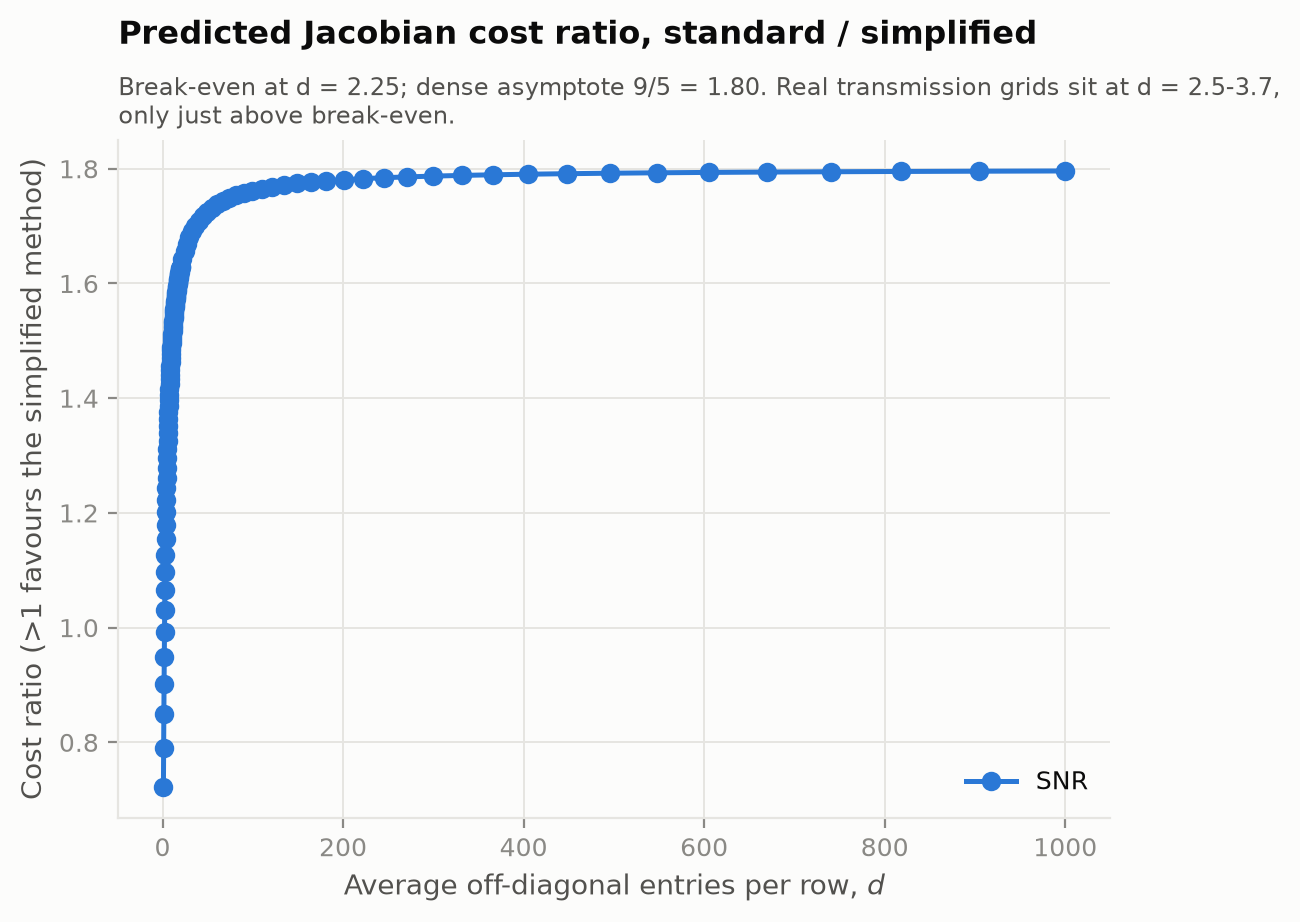
\includegraphics[width=0.72\linewidth]{results/figures/02_ratio_vs_degree.png}
    \caption{Predicted Jacobian cost ratio $r(d)=(9d+4)/(5d+13)$. Break-even at
    $d = 2.25$; dense asymptote $9/5 = 1.80$. Real transmission grids sit at
    $d \approx 2.5$--$3.7$, only just above break-even.}
    \label{fig:ratio-degree}
\end{figure}

The prediction is thus that the simplified method's advantage is real but
modest, that it is largest on a dense formulation such as the paper's, and that
it shrinks to a few per cent once a production-grade sparse solver is used.
This is a sharper statement than the paper makes, and it identifies precisely
the regime in which the method should --- and should not --- be adopted.

\section{Alternative Solution Methods}
Three further solvers were implemented so that the base paper's method could be
placed in a wider context than the single standard-NR baseline it compares
itself against. All of them consume the same \texttt{PowerCase} object and
expose the same entry point, \texttt{solve(case, options, ybus)}, so they are
interchangeable in every experiment; they differ only in the equations they
iterate on.

\subsection{Rectangular Current Injection (RCI)}
The project proposal writes the nodal current injection in rectangular
components, $I_i = \sum_k (G_{ik} + jB_{ik})(e_k + jf_k)$, and forms the
mismatch from its real and imaginary parts. This is \emph{not} what the base
paper does --- the paper keeps the polar state $(|V|,\delta)$ and splits only
the mismatch --- so the proposal's formulation is implemented as a separate
solver in \texttt{solvers/rect\_current\_nr.py}. The unknowns are $(e_k,f_k)$ at
every non-slack bus plus $Q_k$ at every PV bus, and the residuals are
\begin{align}
R^{r}_{k} &= \frac{P_k e_k + Q_k f_k}{e_k^{2}+f_k^{2}}
             - \sum_i \left(G_{ki}e_i - B_{ki}f_i\right), \\
R^{m}_{k} &= \frac{P_k f_k - Q_k e_k}{e_k^{2}+f_k^{2}}
             - \sum_i \left(B_{ki}e_i + G_{ki}f_i\right),
\end{align}
closed at PV buses by the magnitude constraint
$R^{V}_{k} = |V_k^{\mathrm{sch}}|^{2} - (e_k^{2}+f_k^{2})$.

Its attraction is structural and is the same one the base paper is after,
obtained a different way: the network part of the Jacobian is literally $\pm G$
and $\pm B$ taken straight from $Y_{bus}$ and is therefore \emph{constant}. Only
the $2\times2$ diagonal blocks and the PV columns change between iterations, so
an iteration updates $O(n)$ numbers instead of rebuilding the whole matrix ---
a stronger saving than the constant factor of equation~\eqref{eq:ratio-degree}.
The trade-off is the size of the linear system: $2(n-1)+n_{pv}$ against the
paper's $(n-1)+n_{pq}$, which on the $118$-bus system means $287$ unknowns
instead of $181$.

\subsection{Fast Decoupled Load Flow (FDLF)}
FDLF (Stott and Alsa\c{c}, 1974) exploits the weak coupling between $P$
and $|V|$ and between $Q$ and $\delta$ in high-voltage networks. The Jacobian is
replaced once and for all by two constant, real, symmetric matrices built from
the network susceptances,
\begin{equation}
B' \, \Delta\delta = \Delta P / |V|, \qquad
B''\, \Delta|V|    = \Delta Q / |V|,
\end{equation}
which are factorised a single time before the iteration starts. Both standard
variants are implemented, differing in where branch resistance is neglected:
\texttt{XB} drops it from $B'$, \texttt{BX} from $B''$.

FDLF is the natural control for this study. Per iteration it is far cheaper than
either Newton variant --- there is no Jacobian to rebuild at all, which is the
limit the paper's optimisation is approaching --- but it converges only
linearly, so it needs several times more iterations. That trade-off is the point
of including it: the simplified NR method attacks the same cost without giving
up Newton's convergence rate, and FDLF shows what is lost when the cost is
attacked by abandoning that rate instead.

\subsection{Gauss--Seidel (GS)}
Gauss--Seidel is included as the classical baseline the proposal's problem
statement contrasts Newton--Raphson against. Applied bus by bus in place, the
update is the rearranged nodal equation
\begin{equation}
V_k \;\leftarrow\; \frac{1}{Y_{kk}}
    \left[\overline{\left(\frac{S_{\mathrm{sch},k}}{V_k}\right)}
          - \sum_{i \neq k} Y_{ki} V_i \right],
\end{equation}
over-relaxed by an acceleration factor $\alpha = 1.6$. At a PV bus the reactive
injection is first estimated from the present voltages and the updated voltage
is then rescaled back onto its magnitude set-point. It is the cheapest possible
iteration --- no Jacobian, no linear solve, $O(\mathrm{nnz})$ work per sweep ---
and by a wide margin the most expensive method overall, because its convergence
rate degrades as the network grows.

\section{Cross-Method Verification}
Every method must land on the same solution: they differ in the equations they
iterate on, not in the answer. That property is what makes any timing or
iteration-count comparison meaningful, so it is asserted directly in
\texttt{tests/test\_solvers.py} for all seven solvers on all eight test systems.
Each converged solution is checked to zero the \emph{power} mismatch regardless
of the residual it actually iterated on, to respect the slack and PV voltage
set-points, and to agree with a standard-NR reference computed to a
$10^{-12}$ p.u.\ tolerance. Sparse and dense assemblies are checked to agree to
$10^{-8}$ p.u.\ as well. The suite passes in full.

Table~\ref{tab:cross-method} reports the iteration counts. Across the seven
systems no solution differs from the standard-NR reference by more than
$1.1 \times 10^{-7}$ p.u., which is the tolerance the solvers were asked for
rather than a modelling discrepancy.

\begin{table}[H]
\centering
\caption{Iterations to convergence ($10^{-10}$ p.u.\ voltage tolerance;
$10^{-8}$ for Gauss--Seidel). $m$ is the dimension of the linear system solved
each iteration by the polar Newton methods.}
\label{tab:cross-method}
\begin{tabular}{l l r r r r r r r r}
\toprule
{Case} & {System} & {$n$} & {$m$} & {SNR} & {PNR} & {PNR+} & {RCI} & {FDLF} & {GS} \\
\midrule
TC1 & case5\_stagg      & 5   & 8   & 5 & 5  & 5 & 4 & 9  & 39      \\
TC2 & case6ww           & 6   & 8   & 4 & 8  & 5 & 4 & 12 & 35      \\
TC3 & case24\_ieee\_rts & 24  & 36  & 5 & 9  & 6 & 6 & 10 & 107     \\
TC4 & case30\_ieee      & 30  & 53  & 5 & 7  & 5 & 5 & 13 & 153     \\
TC5 & case57\_ieee      & 57  & 106 & 5 & 10 & 5 & 5 & 11 & 164     \\
EX1 & case118\_ieee     & 118 & 181 & 5 & 19 & 6 & 6 & 13 & 573     \\
EX2 & case300\_ieee     & 300 & 530 & 6 & 21 & 7 & 7 & 18 & 8\,716  \\
\bottomrule
\end{tabular}
\end{table}

Three observations follow, and together they frame the cost analysis above.

First, the base paper's method (PNR) consistently needs \emph{more} iterations
than the standard method, and the gap widens with system size --- $19$ against
$5$ at $118$ buses, $21$ against $6$ at $300$. This is the direct cost of
lagging the PV-bus reactive power behind the voltage estimate, which layers a
successive-substitution fixed point on top of Newton's method and destroys its
quadratic rate. The augmented variant (PNR+), in which $Q$ becomes a genuine
Newton unknown, restores it: it stays within one iteration of standard NR on
every system tested.

Second, the modest per-iteration saving established in
Table~\ref{tab:sparse-flops} --- around $15\%$ on a sparse implementation ---
cannot pay for a fourfold increase in iteration count. The paper's claim is
sound at the level at which it is made, the cost of a single Jacobian rebuild,
and does not survive being carried through to end-to-end solution time unless
the PV handling is fixed as well.

Third, RCI matches or beats standard NR on iteration count everywhere, which is
expected of a full Newton method with an exact Jacobian, while FDLF needs two to
three times as many and Gauss--Seidel one to three orders of magnitude more.
The ordering confirms that the four solvers span the intended range of the
cost-per-iteration against iterations-to-convergence trade-off.


\end{document}
